\documentclass[12pt, a4paper, onecolumn]{report}
%  \usepackage[english, brazilian, portuges]{babel}
  \usepackage[brazilian]{babel}
  \usepackage[T1]{fontenc}
  \usepackage{ae}
  \usepackage[utf8]{inputenc}
  \usepackage{graphicx, subfig}
  \usepackage{algorithm, algorithmic}
  \usepackage{listings}
  \usepackage{amsmath}
  \usepackage{amsthm}
  \usepackage{listings}
  \usepackage{setspace}
  \usepackage{indentfirst}
  \usepackage{lscape}
  \usepackage[toc,page]{appendix}
  \usepackage[a4paper]{geometry}
  \geometry{hmargin={3cm,2cm}}
  \geometry{vmargin={3cm,2cm}}
  \newtheorem{mprocessamentoydef}{Definição}
  \graphicspath{{images//}}
  \renewcommand{\appendixtocname}{Apêndices}
  \renewcommand{\appendixpagename}{Apêndices}
  \renewcommand{\listalgorithmname}{Lista de pseudo-algoritmos}


\begin{document}
\begin{titlepage}
  \begin{minipage}{0.2\linewidth}

%  \begin{figure}[h!]
%    \begin{center}
      
\includegraphics[width=0.8\textwidth]{minerva.jpg}
%      \centering
%      \caption{Distância vertical.}
%    \end{center}
%  \end{figure}

  \end{minipage}
  \begin{minipage}{0.8\linewidth}
    \textbf{Universidade Federal do Rio de Janeiro} \\
    Instituto de Matemática \\
    Departamento de Ciência da Computação \\
    Rio de Janeiro, RJ - Brasil\\
    \rule{0.8\linewidth}{0.2mm}\\

  \end{minipage}

  \begin{center}
  \vspace{4cm}
  \Large
  Aplicação do algoritmo \textit{Perceptually Important Points} em séries temporais de datacenters
  \end{center}

  \begin{center}
  \vspace{0.25cm}
  \normalsize
  Ronald Andreu Kaiser \\
  %\vspace{cm}
  Orientadora: \\Adriana Santarosa Vivacqua
  \end{center}
  \vfill

  \begin{center}
  Dezembro de 2010
  \end{center}

  \vspace{2cm}
\end{titlepage}

\begin{titlepage}
  \begin{center}
    \large
    Aplicação do algoritmo \textit{Perceptually Important Points} em séries temporais de datacenters\\
    \vspace{1cm}
    \normalsize
    Ronald Andreu Kaiser \\
  \end{center}
\flushleft
Projeto Final de Curso submetido ao Departamento de Ciência da Computação do Instituto de Matemática da Universidade Federal do Rio de Janeiro como parte dos requisitos necessários para obtenção do grau de Bacharel em Informática. \\

\vspace{1cm}
Apresentado por: \\
\flushright
\_\_\_\_\_\_\_\_\_\_\_\_\_\_\_\_\_\_\_\_\_\_\_\_\_\_\_\_\_\_\_\_\_\_\_\_\_\_\_\\
Ronald Andreu Kaiser

\vspace{1cm}
\flushleft
Aprovado por: \\
\flushright
\_\_\_\_\_\_\_\_\_\_\_\_\_\_\_\_\_\_\_\_\_\_\_\_\_\_\_\_\_\_\_\_\_\_\_\_\_\_\_\\
Adriana Santarosa Vivacqua\\
D.Sc. COPPE/UFRJ

\vspace{1cm}
\_\_\_\_\_\_\_\_\_\_\_\_\_\_\_\_\_\_\_\_\_\_\_\_\_\_\_\_\_\_\_\_\_\_\_\_\_\_\_\\
João Carlos Pereira da Silva \\
D. Sc. UFRJ

\vspace{1cm}
\_\_\_\_\_\_\_\_\_\_\_\_\_\_\_\_\_\_\_\_\_\_\_\_\_\_\_\_\_\_\_\_\_\_\_\_\_\_\_\\
Marcello Goulart Teixeira \\
D. Sc. PUC-Rio

\vfill

\begin{center}
RIO DE JANEIRO, RJ - BRASIL\\
Dezembro de 2010
\end{center}

\vspace{2cm}
\end{titlepage}

\singlespace
\begin{titlepage}
\begin{center}
  \Large
  \textbf{Agradecimentos}
\end{center}

Agradeço a todo o Universo, por ter se organizado de tal maneira que fosse possível a realização desse projeto. Obrigado por sua complexidade, que torna nossas vidas menos enfadonhas e previsíveis.

Agradeço a minha mãe, Monique E. C. D. Nitsche, por ter me ajudado a experimentar a vida e por sua luta em dar o melhor de si para que eu pudesse sobreviver e alcançar meus objetivos.

Agradeço a minha tia Vera Sarres, por ter aturado minhas excentricidades por esses anos e me dado abrigo e conforto.

Agradecimento especial aos amigos da casa Intelie, Ricardo Clemente, Pedro Teixeira, Hubert Fonseca e o grande Falcão pelo apoio e incentivo que vocês me deram durante todo o tempo que nos conhecemos. Obrigado pelas grandes lições de vida e experiências que vocês me proporcionaram. Obrigado pela oportunidade que foi fundamental para realização deste trabalho e a compreensão nos momentos que precisei me ausentar para terminá-lo. Serei eternamente grato a vocês.

Agradeço a Anna Cruz pelas conversas e por ter me ajudado a tirar alguns screenshots para a versão final e ao Rodolfo Carvalho, pelas coisas que aprendi com ele.

Agradeço a minha orientadora, Adriana S. Vivacqua, por ter aceitado esse desafio, seu incentivo e indispensável ajuda nesse trabalho.

Agradeço a UFRJ por, apesar de todos os seus defeitos, prezar pelo ensino de qualidade e excelência de computação.

Agradeço ao Tiago S. da Silva, por sua amizade e pelos papos filosóficos que tivemos durante o curso.

Agradeço a Adriana Pinho pelas prazerosas conversas sobre ciência e sociedade, além de conselhos para essa monografia.

Agradeço também a todas as inúmeras pessoas e situações que me ajudaram direta ou indiretamente a ser uma pessoa melhor.


\end{titlepage}

\begin{titlepage}
\begin{center}
  \Large
  \textbf{Resumo}
\end{center}
Kaiser, R. A. Aplicação do algoritmo \textit{Perceptually Important Points} em séries temporais de datacenters.\\

O propósito deste trabalho é auxiliar operadores de datacenters na visualização de gráficos de séries temporais, que representam a evolução do comportamento de seus equipamentos e serviços. Para tanto, foi buscada inspiração em um algoritmo utilizado para o reconhecimento de padrões em séries temporais do mercado financeiro. O algoritmo \textit{Perceptually Important Points} ao mesmo tempo que contribui para a redução de dimensionalidade, fornece um mecanismo automatizado de eleição dos pontos mais importantes de uma série temporal para um observador humano, favorecendo, deste modo, sua visualização e tráfego pela rede. A implementação do algoritmo e sua implantação em um sistema de monitoração de datacenters já existente, hoje utilizado por grandes datacenters do Brasil, constituem o cerne deste trabalho. \\

\textbf{Palavras-Chave:} Séries Temporais, Redução de dimensionalidade, Perceptually Important Points, Datacenters, Clojure.

\end{titlepage}

\begin{titlepage}
\begin{center}
  \Large
  \textbf{Abstract}
\end{center}
Kaiser, R. A. Aplicação do algoritmo \textit{Perceptually Important Points} em séries temporais de datacenters.\\

The main purpose of this work is helping operators of datacenters in the task of visualizing the behaviour of their devices and services through time, represented by large time series. In order to accomplish that, a technique used in pattern recognition from the financial market context was choosed. The ``Perceptually Important Points'' algorithm gives a method for dimensionality reduction and a mechanism to automatically extract the most important points from a human observer perspective, favouring compression and a good visualization of time series with high dimensionality. The implementation of the algorithm and its integration in an existing monitoring system was explored and encompasses the content of this work.\\

\textbf{Keywords:} Time series, Dimensionality Reduction, Perceptually Important Points, Datacenters, Clojure.

\end{titlepage}

\listoffigures
\listoftables
\listofalgorithms
\tableofcontents

\onehalfspacing
\chapter{Introdução}
\label{chap:introducao}

Manter sistemas complexos em pleno funcionamento e harmonia requer constante monitoração de suas partes. Datacenters, por menores que sejam, precisam ser constantemente monitorados para garantir que seus equipamentos e serviços estejam disponíveis e em correto funcionamento. Nesses ambientes, subutilização de recursos, períodos de inatividade ou falhas em dispositivos são situações indesejáveis que podem levar a perdas de faturamento significativas por parte de seus mantenedores.

Para evitar tais riscos, medições sobre equipamentos e serviços precisam ser coletadas continuamente com o objetivo de apoiar a tomada de decisão, tanto em níveis micro, onde simples mudanças de dispositivos são agendadas, até reestruturações em arquiteturas de serviços. 

Datacenters podem ser vistos como verdadeiras ``máquinas'' de produção de séries temporais. Como medições são realizadas com frequência, é natural observar nesse contexto séries temporais com alta dimensionalidade representadas por \textit{datasets} de muitos gibibytes de aglomerados numéricos semi-estruturados. É desejável, portanto, que se tenha um meio apropriado de visualização de dados e entre outras formas de leitura, a visualização de gráficos desempenha um papel importante.

O propósito deste trabalho é auxiliar operadores de datacenters na recuperação e visualização de gráficos, que representam a evolução do comportamento de seus equipamentos e serviços, e para tanto foi buscada inspiração em um algoritmo utilizado para o reconhecimento de padrões em séries temporais do mercado financeiro. 

O algoritmo \textit{Perceptually Important Points}\footnote{Preferiu-se o termo \textit{Perceptually Important Points} em sua língua inglesa por ser mais conhecido dessa forma na literatura, além de oferecer o mneumônico e acrônimo PIP.} ao mesmo tempo que contribui para a redução de dimensionalidade, fornece um mecanismo automatizado de eleição dos pontos mais importantes de uma série temporal para um observador humano, favorecendo, deste modo, sua visualização e tráfego pela rede.

A implementação do algoritmo e sua implantação em um sistema de monitoração de datacenters já existente\footnote{O software citado recebe o nome de HOLMES e será apresentado no capítulo \ref{chap:holmes}.}, hoje utilizado por grandes datacenters do Brasil, constituem o cerne deste texto. 

Nas próximas seções são apresentadas as motivações que fomentaram a elaboração deste trabalho, os objetivos pretendidos, a metodologia aplicada e um resumo de cada capítulo foi acrescentado para que o leitor possa obter uma visão geral da organização deste texto.


\section{Motivação}
\label{sec:motivacao}
Softwares atuais largamente utilizados no contexto de datacenters, como RRDtool~\cite{rrdtool} se baseiam em funções agregadoras simples de média, máximo ou mínimo, que podem deturpar a interpretação de seus gráficos.

A motivação deste trabalho é a de solucionar a carência de um mecanismo eficaz para a representação e visualização de séries temporais em um software de monitoração de datacenters, a saber, HOLMES.

O sistema HOLMES conta com uma interface web, onde o usuário final, em geral, um operador de datacenter, tem a capacidade de visualizar o comportamento de um de seus equipamentos ou serviços ao longo do tempo. Para tanto, o usuário faz requisições HTTP a séries temporais via REST\footnote{REST, Representational State Transfer, técnica de engenharia de software para sistemas hipermídia distribuídos. Comumente usada no contexto da World Wide Web.}.

Responder a essas requisições com os dados originais pode provocar alguns problemas, tais como:

\begin{itemize}
\item Perdas de performance causadas pelo tráfego de milhares de pontos pela rede;
\item Gráficos com muitos pontos em uma área reduzida pode favorecer representações muito densas, visualmente poluídas e pouco informativas;
\item Consumo de memória excessivo para o usuário final, dado que os pontos são armazenados no web browser do cliente.
\end{itemize}

\section{Objetivos}
\label{sec:objetivos}
A fim de solucionar os problemas mencionados na seção anterior, os objetivos traçados para a realização deste trabalho incluem:
\begin{enumerate}
  \item Implementar um algoritmo que reduza a dimensionalidade de séries temporais e represente visualmente de modo mais fiel possível as séries originais;
  \item Integração em um software de monitoração de datacenters.
\end{enumerate}

\section{Metodologia}
Para fins de execução dos desafios propostos, fez-se necessário o estudo e pesquisa de artigos e livros na área de séries temporais. Fundamentado nesse estudo, optou-se por implementar o algoritmo \textit{Perceptually Important Points} por ser conceitualmente simples e atender de forma satisfatória no domínio aplicado.

Como o algoritmo escolhido apresentava complexidade de tempo $O(n^2)$, questões de performance e desempenho foram trabalhadas e viabilizar a implementação do código-fonte requereu um estudo mais aprofundado sobre a linguagem de programação Clojure. 

Vale ressaltar também que desde o princípio deste projeto foi vislumbrada a implantação do algoritmo em um software de monitoração de datacenters e sua arquitetura e integração com o algoritmo escolhido foi pensada e analisada durante todo o processo.

\section{Organização da Monografia}

\begin{itemize}

\item O capítulo \ref{chap:time-series} contribui com um apanhado sobre o que existe na literatura sobre séries temporais objetivando fundamentar as bases teóricas para o desenvolvimento dos próximos capítulos. Modelos de representação e características de séries temporais são apresentados, além de contextualizações com a realidade de datacenters típicos.

\item O capítulo \ref{chap:pip} apresenta o algoritmo \textit{Perceptually Important Points}, escolhido para implementação neste trabalho. A intuição por trás do método é revelada, junto com seu pseudo-algoritmo, análise de complexidade, limitações e comparações com métodos existentes.

\item O capítulo \ref{chap:implementacao} expõe uma instância do algoritmo \textit{Perceptually Important Points} implementada na linguagem Clojure. Detalhes de implementação, características do código gerado, dificuldades e testes de performance realizados são apresentados.

\item O capítulo \ref{chap:holmes} demonstra como se realizou a integração do algoritmo descrito no capítulo \ref{chap:implementacao} em um software de monitoração de datacenters. Seu propósito e uma visão geral da arquitetura do sistema envolvida na integração do algoritmo é discutida, seguida de um caso de uso de sucesso.

\item Por fim, no capítulo \ref{chap:conclusao} seguem as conclusões sobre o trabalho realizado e propostas de trabalhos futuros são delineadas.
\end{itemize}

\chapter{Séries temporais}
\label{chap:time-series}
Na área médica, é comum a monitoração da evolução de funções vitais de pacientes através de aparelhos como eletroencefalogramas e eletrocardiogramas, além do acompanhamento da incidência de padrões sazonais de epidemias~\cite{metodosmedicina}. Na ciência econômica, muitos livros~\cite{forecastingeconomic} e artigos~\cite{germantimeseries} já foram escritos sobre análises e previsões do mercado financeiro, políticas fiscais e monetárias, baseadas em observações no tempo. O que a Medicina e a Economia e outras áreas supostamente não correlatas possuem em comum é o fato de permitirem a aplicação de estudos e métodos de séries temporais.

Séries temporais podem ser construídas sobre praticamente quaisquer medições possíveis no tempo e esse caráter genérico é o que torna a utilidade do seu estudo indiscutível em diversas áreas do conhecimento humano. O tema é usado com sutis diferenças entre matemáticos, estatísticos e outros profissionais. Por essa razão, segue a definição que será utilizada\footnote{Séries temporais também podem ser definidas como um conjunto de observações $\{X(t), t \in T\}$, com $X$ representando a variável aleatória observada e T um conjunto de índices.}:


\theoremstyle{definition}
\newtheorem{time-series}{Definição}
\begin{time-series}
Série temporal: sequência de observações\footnote{Tais observações podem ser coletadas em períodos regulares ou não.} ordenadas cronologicamente (n-tupla):
\begin{equation}\label{eq:time-series}
 \\S = (s_{1}, s_{2}, s_{3}, ..., s_{n})
\end{equation}
\end{time-series}

  \begin{figure}
    \begin{center}
      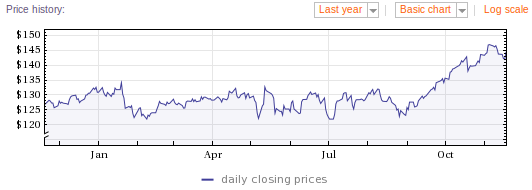
\includegraphics[width=0.9\textwidth]{ibm_stock}
      \centering
      \caption[Preço de fechamento de ações da IBM - 2010.]{Preço de fechamento de ações da IBM no ano de 2010~\cite{wolframalpha}.}
    \label{fig:ibm-stock}
    \end{center}
  \end{figure}

Quando tais observações são coletadas no tempo continuamente, diz-se que a série temporal é \textit{contínua} e quando as medições se fazem em instantes de tempo específicos, geralmente equidistantes, são conhecidas como séries temporais \textit{discretas}. 

Na figura \ref{fig:ibm-stock}, podemos visualizar um exemplo de série temporal discreta, descrevendo o preço de fechamento das ações da IBM ao longo do ano de 2010.

Em geral, o estudo de séries temporais comporta objetivos dos mais diversos, como identificação de tendências e outliers\footnote{Observações distantes ou discrepantes quando comparadas globalmente com outras observações.}, predição, similaridade entre séries temporais por clusterização, existência de sazonalidades -- endereçado na seção \ref{sub:sazonalidade} -- entre outros.

A seguir, serão apresentadas características e técnicas envolvidas na visualização, representação e análise de séries temporais. Ao final deste capítulo, contextualizaremos o papel de séries temporais com a realidade de grandes datacenters.

\section{Características}
\subsection{Dependência de observações}
O valor das ações da IBM ao final de um dia se torna naturalmente dependente do seu desempenho em dias anteriores. Da mesma forma, o número de pessoas que habitavam o planeta Terra em anos passados tem influência direta sobre a população mundial de hoje.

É comum encontrar na literatura~\cite{timeseriesr}, ressalvas sobre a aplicação de muitos métodos estatísticos tradicionalmente baseados na suposição de que observações adjacentes são independentes e identicamente distribuídas. Sendo assim, identificar a existência de correlações entre medições no tempo é essencial para que possamos aplicar análises estatísticas apropriadas.

\subsection{Alta dimensionalidade}
\label{sub:alta-dimensionalidade}
É comum observar na literatura a interpretação da n-tupla descrita na definição \ref{eq:time-series} como um ponto em uma espaço de dimensão $\Re^n$. Como novas observações são coletadas constantemente, séries temporais assumem, portanto, caráter de alta dimensionalidade.

Como possuem centenas de milhares a milhões de pontos e tratá-los em sua forma bruta se torna computacionalmente custoso, é desejável, em aplicações práticas, um mecanismo que favoreça a redução de dimensionalidade.

\subsection{Sazonalidade}
\label{sub:sazonalidade}
É possível identificar na Natureza diversos fenômenos que possuem algum comportamento sazonal. A produção de arroz na China, o número de passagens vendidas por uma companhia aérea ao longo de um ano, a migração das aves com a chegada do inverno e a quantidade de visitas em uma página na Internet possuem no mínimo um comportamento em comum: sazonalidade.

No contexto de séries temporais, o termo \textit{sazonalidade} diz respeito a padrões que se repetem em períodos no tempo. Sazonalidades podem ser classificadas em dois tipos: aditivas e multiplicativas. A primeira retrata flutuações que não sofrem mudanças muito bruscas quando considerada a série globalmente. Sazonalidades multiplicativas dependem de um fator em cada período em que é observada e possuem uma maior variabilidade quando comparadas com a série original como um todo.

\subsection{Tendência}
A quantidade de água doce no mundo vem diminuindo ao longo dos anos. Ao mesmo tempo, o número de artigos científicos publicados no meio acadêmico cresce monotonicamente. Tendências de crescimento ou decrescimento podem ser identificadas em séries temporais e podem ser caracterizadas por sua taxa de variação. Se sua taxa de crescimento se aproximar de uma reta, diz-se que a série possui tendência linear. Caso contrário, tendências podem ser classificadas como não lineares, exponenciais ou quadráticas.


\begin{figure}[htb!]
  \begin{center}
    \subfloat[Sem tendência ou sazonalidade]{\label{fig:ts0}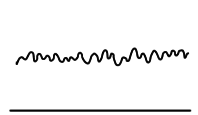
\includegraphics[width=0.25\textwidth]{tend-sazonalidade0}} \quad
    \subfloat[Sem tendência, com sazonalidade]{\label{fig:ts1}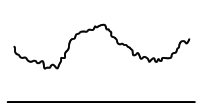
\includegraphics[width=0.25\textwidth]{tend-sazonalidade1}} \quad
    \subfloat[Tendência linear, com sazonalidade aditiva]{\label{fig:ts2}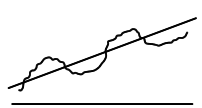
\includegraphics[width=0.25\textwidth]{tend-sazonalidade2}}
    \\
    \subfloat[Tendência linear e sazonalidade multiplicativa]{\label{fig:ts3}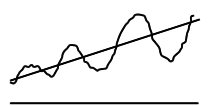
\includegraphics[width=0.25\textwidth]{tend-sazonalidade3}} \quad
    \subfloat[Tendência não linear e sazonalidade aditiva]{\label{fig:ts4}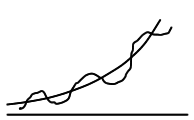
\includegraphics[width=0.25\textwidth]{tend-sazonalidade4}} \quad
    \subfloat[Tendência não linear e sazonalidade multiplicativa]{\label{fig:ts5}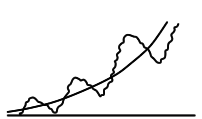
\includegraphics[width=0.25\textwidth]{tend-sazonalidade5}}
    \centering
    \caption{Padrões de tendência e sazonalidade em séries temporais}
  \label{fig:tend-sazonalidade}
  \end{center}
\end{figure}

Na figura \ref{fig:tend-sazonalidade}, padrões de comportamento relacionando sazonalidade e tendência podem ser observados. Além das características apresentadas, outras bastante utilizadas na literatura e não menos importantes são  estacionariedade, aleatoriedade e ciclidade. A seguir, uma breve descrição de técnicas largamente utilizadas para análise e compressão de séries temporais.

\section{Representação e redução de dimensionalidade}
A representação de séries temporais em sua forma original pode ser computacionalmente custosa, dada sua alta dimensionalidade -- discutida na seção \ref{sub:alta-dimensionalidade}. A escolha do método de representação deve se basear na aplicabilidade desejada. Existem atualmente diversas abordagens para compressão e representação de séries temporais. Algumas se baseiam em transformações de domínios, como \textit{Discrete Fourier Transform}, que mapeiam para o domínio de frequências uma série em seu domínio temporal, outras podem preservar dois domínios, como é o caso de \textit{Discrete Wavelet Transform}. O objetivo dessa seção é apresentar as ideias das abordagens mais conhecidas e utilizadas.

\subsection{Algoritmos utilizados}
Séries temporais podem ser vistas como funções matemáticas e como tais podem se favorecer de técnicas básicas da Matemática Aplicada, como aproximações de funções complexas por funções mais simples, como retas. O método conhecido como PLA (Piecewise Linear Approximation) segmenta uma série temporal em partes e para cada uma delas define a reta que mais se aproxima dos pontos no segmento considerado. Na figura \ref{fig:pla} podemos ver um exemplo de como uma série pode ser aproximada por esse método.

  \begin{figure}[htb!]
    \begin{center}
      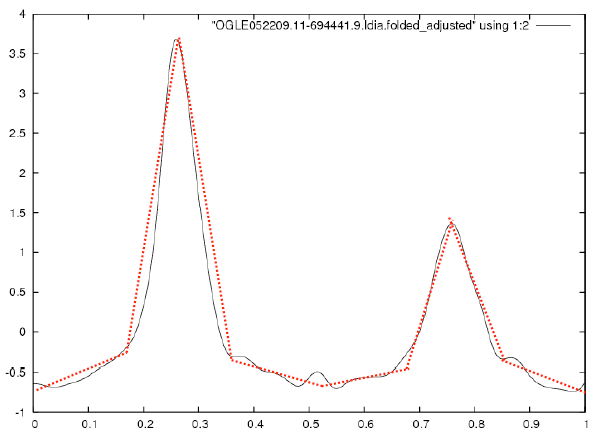
\includegraphics[width=0.6\textwidth]{pla}
      \centering
      \caption{Piecewise Linear Approximation}
    \label{fig:pla}
    \end{center}
  \end{figure}

Abordagens com teor matemático mais apurados também são utilizadas para representar séries temporais. Os resultados de Jean-Baptiste Joseph Fourier, que demonstrou que todo sinal periódico poderia ser aproximado por somas de senos e cossenos, podem ser mapeados para o campo dos números complexos, dando origem a transformada de Fourier.

  \begin{figure}[htb!]
    \begin{center}
      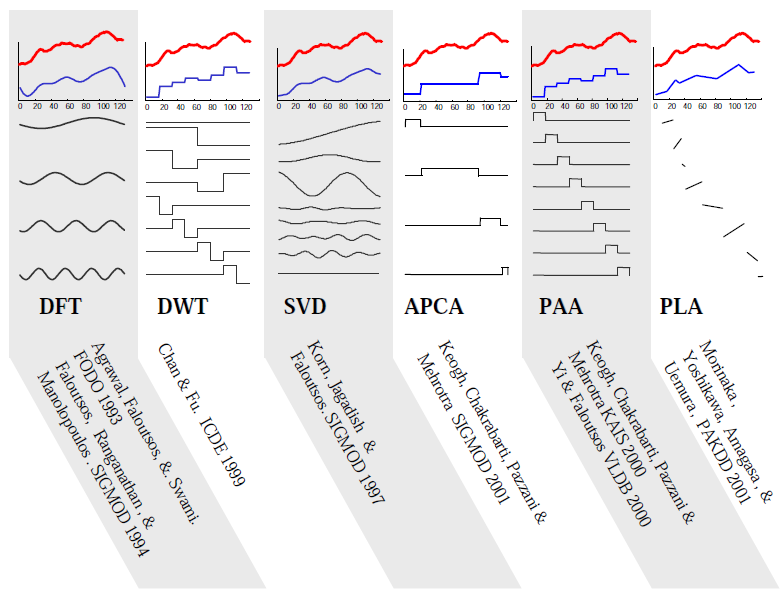
\includegraphics[width=1\textwidth]{comparing_methods}
      \centering
      \caption[Comparação entre algoritmos de representação.]{Comparação entre algoritmos de representação e redução de dimensionalidade de séries temporais.}
    \label{fig:comparing-methods}
    \end{center}
  \end{figure}

A partir dessa transformada, uma série temporal pode ser decomposta por suas componentes no domínio das frequências. Na primeira coluna da figura \ref{fig:comparing-methods} podemos ver como uma aproximação pode ser feita com o algoritmo FFT (Fast Fourier Transform), uma das variantes de uma classe maior de algoritmos baseados na transformada de Fourier, conhecida como DFT (Discrete Fourier Transform). Uma desvantagem deste método é que se perde o referencial de eventos no tempo, tendo que se recorrer a transformada inversa de Fourier~\cite{dftandwavelets}.

Outro algoritmo largamente utilizado para compressão de imagens e que pode ser utilizado para redução de dimensionalidade de séries temporais é o DWT (Discrete Wavelet Transform), mais vantajoso do que o DFT em alguns aspectos, pois preserva componentes no domínio do tempo~\cite{insightintowavelets}. Uma ``wavelet'' ou ondaleta é uma pequena onda que pode ser usada como base para a reconstrução da série original e diferente dos senos e cossenos utilizados no DFT não podem ser funções periódicas. Para a utilização desse algoritmo é necessário que se escolha previamente duas ondaletas, normalmente conhecidas como ondas mãe $\psi$ e pai $\phi$ que devem satisfazer alguns critérios de ortogonalidade. 

  \begin{figure}[htb!]
    \begin{center}
      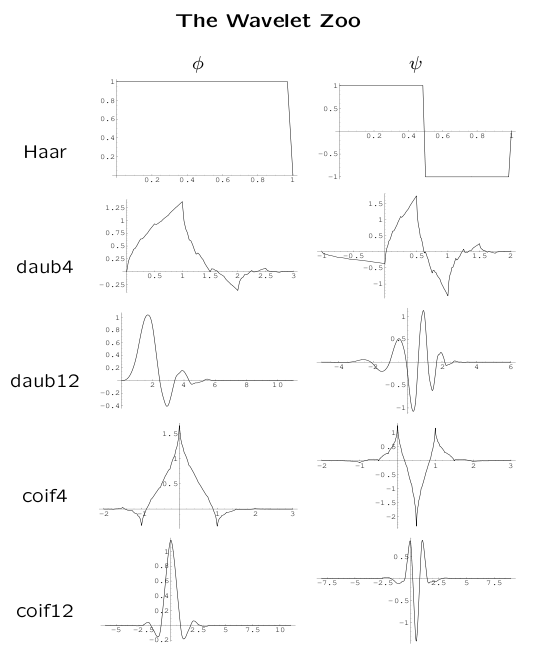
\includegraphics[width=0.7\textwidth]{zoo}
      \centering
      \caption{Família de Wavelets.}
    \label{fig:zoo}
    \end{center}
  \end{figure}



Na figura \ref{fig:zoo} podemos ver pares de funções mãe e pai que satisfazem esses critérios e podem ser utilizadas como wavelets. Repare na segunda coluna da figura \ref{fig:comparing-methods} a aproximação de uma série utilizando a ondaleta Haar, reconhecida como a primeira ondaleta utilizada.

Ainda na figura \ref{fig:comparing-methods}, pode-se observar como os métodos apresentados e outros se comportam para a mesma série original de entrada. Em cada coluna, a série original de entrada aparece em vermelho e logo abaixo, em azul, a série aproximada pelo algoritmo correspondente. Comparações mais detalhadas sobre DFT e DWT podem ser encontradas em~\cite{dftandwavelets}.

Além dos apresentados, existem na literatura diversos algoritmos de representação e redução de dimensionalidade de séries temporais. Alguns deles são: Piecewise Constant Approximation (PCA), Symbolic Approximation (SA), Symbolic Aggregate ApproXimation (SAX), Singular Value Decomposition (SVD), CHEByshev polynomials (CHEB) e Self-Organizing Maps (SOM).

A partir dessa visão geral sobre o atual cenário no que diz respeito a representação e compressão de séries temporais, na próxima seção uma contextualização com o ambiente de datacenters será apresentada.

\section{Séries temporais de datacenters}
\label{sec:time-series-datacenter}
Datacenters são ambientes que concentram equipamentos de processamento e armazenamento de dados de empresas ou organizações. Podem ser considerados como legítimas ``máquinas'' de produção de séries temporais. Em uma instalação típica, são encontrados diversos racks de servidores centralizadores de inúmeras unidades de processamento e armazenamento.

O foco deste trabalho se concentra em séries temporais de observações feitas sobre os equipamentos e dispositivos desses datacenters. O operador de um grande datacenter, em geral, precisa monitorar dados de consumo de CPU, memória, sessões TCP abertas, requisições HTTP, taxa de hits em caches, número de consultas lentas a bancos de dados, entre outras métricas. Em datacenters possuímos um conjunto bem heterogêneo de padrões de séries temporais. Na figura \ref{fig:series-temporais-datacenter} podemos ver alguns exemplos de gráficos que fazem parte do dia a dia de operação de um datacenter. 

Esses gráficos foram gerados através de uma ferramenta bem conhecida, RRDtool. Com essa ferramenta é possível escrever scripts para coletar informações de dispositivos de tempos em tempos. O software é livre e utiliza o conceito de Round Robin Database, em que é mantido sempre uma quantidade fixa de pontos de cada série. Quando o limite é ultrapassado, algumas estratégias podem ser definidas. A mais simples de todas é descartar sempre os pontos mais antigos. Pode-se também configurar cálculos de agregados, resumindo pontos por sua média, mínimo ou máximo. 

Essa abordagem nem sempre é satisfatória na busca por uma causa para uma possível falha em um desses equipamentos, pois médias em dados com variância muito alta podem mascarar falhas graves. É desejável, portanto, que se tenha uma forma eficiente de visualização que permita capturar características apresentadas nesse capítulo, como sazonalidades e tendências. Essas observações é que permitirão coletar fatos e reorganizar a estrutura do datacenter para que o mesmo se mantenha em pleno funcionamento. Para tanto, algum dos algoritmos de representação e redução de dimensionalidade se faz necessário. 

No próximo capítulo veremos as ideias que estão por trás do algoritmo \textit{Perceptually Important Points}, seguido de sua implementação e a contextualização com datacenters será retomada no capítulo \ref{chap:holmes}, que retratará a aplicação do algoritmo em um sistema real de monitoração.

\begin{figure}[htb!]
  \begin{center}
    \subfloat[Consumo de CPU]{\label{fig:cpu}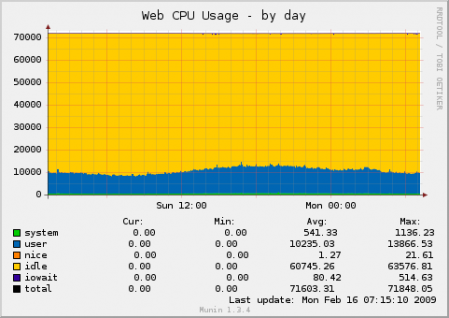
\includegraphics[width=0.7\textwidth]{cpu}}
    \\
    \subfloat[Tráfego de rede]{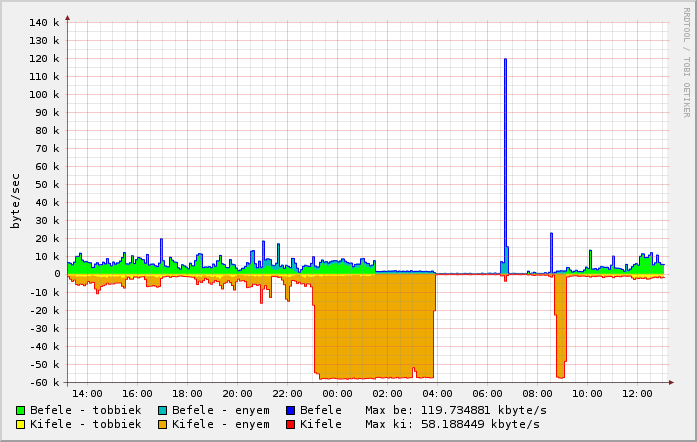
\includegraphics[width=0.7\textwidth]{network_day}}
    \\
    \subfloat[Uso do protocolo SMPP em um roteador]{\label{fig:pip2}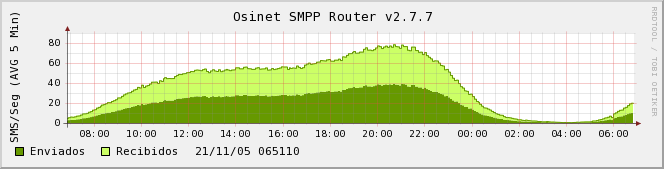
\includegraphics[width=0.7\textwidth]{smpp_router}}
    \\
    \centering
    \caption{Gráficos típicos no dia a dia de operação de um datacenter}
    \label{fig:series-temporais-datacenter}
  \end{center}
\end{figure}


\chapter{Perceptually Important Points}
\label{chap:pip}

Para atingir o primeiro objetivo -- proposto na seção \ref{sec:objetivos} --, escolheu-se o algoritmo \textit{Perceptually Important Points}, pois se mostrou conceitualmente simples em relação aos outros métodos apresentados no capítulo anterior, além de favorecer uma forma eficaz na redução de dimensionalidade de séries temporais.

\section{Ideia do algoritmo}
A primeira proposta formal do processo de identificação de \textit{Perceptually Important Points} foi introduzida por~\cite{firstpip} em uma análise técnica de padrões para aplicações financeiras, com ideias parecidas utilizadas em trabalhos independentes de~\cite{perng2000} e ~\cite{fink2003}. Entretanto, não é conhecida a utilização dessa técnica para o auxílio da representação de séries temporais de datacenters.

O algoritmo expressa um método para se definir que pontos são de fato imprescindíveis e que devem ser considerados para que a plotagem do gráfico preserve sua forma original para um observador humano.


Para ilustrar a ideia do algoritmo, vamos utilizar como série base, uma amostra de 50 pontos de uma função seno multiplicada por um fator aleatório entre 0 e 5 -- para incluir algum ruído nos dados, ilustrada na figura \ref{fig:original}.

Para podermos identificar os pontos mais importantes de uma série, é preciso considerá-la como um todo. Alguns pontos podem ser importantes em um período, mas completamente descartáveis quando se considera toda a sua história. Por essa razão, faz parte da inicialização do algoritmo incluir o primeiro e último pontos da série original, veja figura \ref{fig:inicializacao-pip}. 

Em sua primeira iteração, calculamos a distância de todos os pontos no intervalo com relação aos primeiros pontos escolhidos na inicialização. O ponto que possuir maior distância dos dois primeiros será o próximo ponto a ser promovido a PIP.

Após a primeira iteração, processamos todas as distâncias, agora para os dois intervalos implícitos pelos 3 pontos já escolhidos. Escolhemos nessa iteração o ponto que possui a maior distância desses intervalos e o promovemos a PIP. O processo se repete até que todos os pontos sejam escolhidos e estejam devidamente ordenados. 

Outros procedimentos e condições de parada podem ser definidos, como por exemplo, um valor fixo para o número de pontos a serem escolhidos, ou a atribuição de um erro tolerável. Tais condições serão discutidas ainda neste capítulo na seção \ref{sec:pseudo-algoritmo}.

\begin{figure}[htb!]
  \begin{center}
    \subfloat[Série original com 50 pontos.]{\label{fig:original}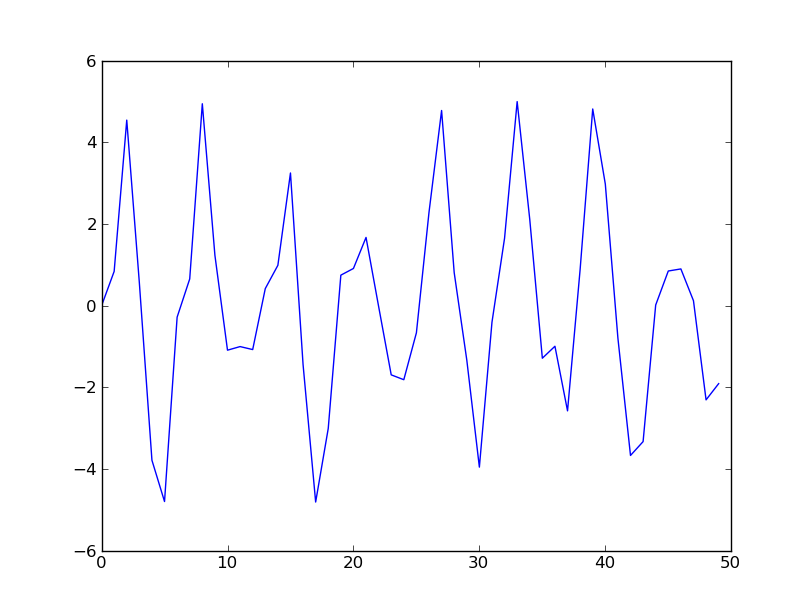
\includegraphics[width=0.5\textwidth]{original}}
    \\
    \subfloat[Inicialização.]{\label{fig:inicializacao-pip}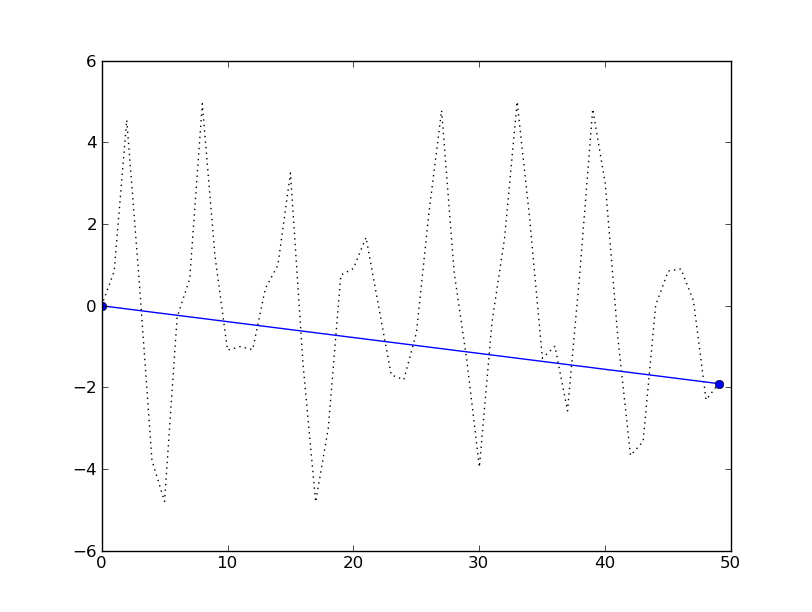
\includegraphics[width=0.4\textwidth]{pip2}}
    \subfloat[5 PIPs.]{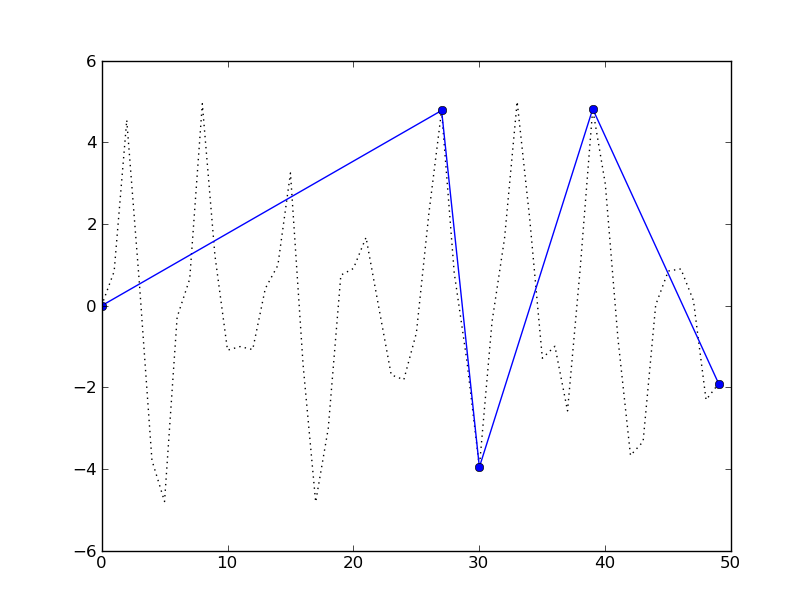
\includegraphics[width=0.4\textwidth]{pip5}}
    \\
    \subfloat[10 PIPs.]{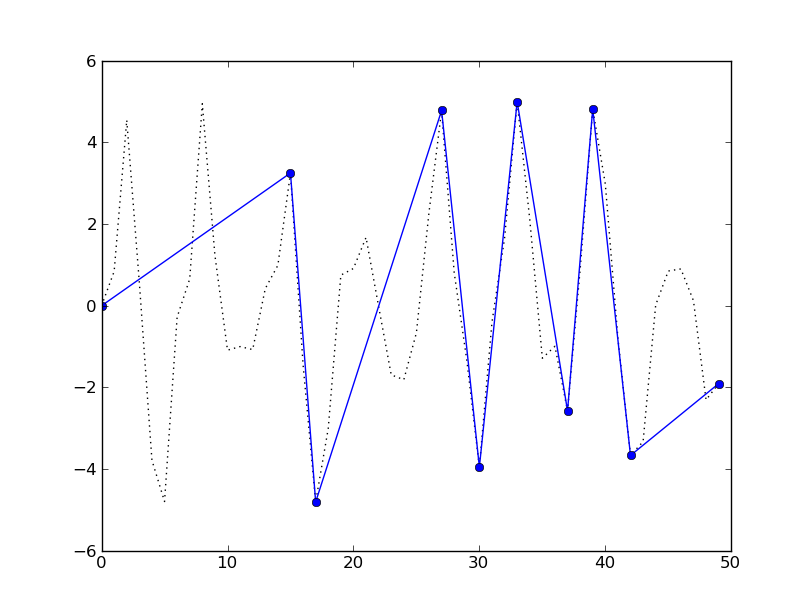
\includegraphics[width=0.4\textwidth]{pip10}}
    \subfloat[20 PIPs.]{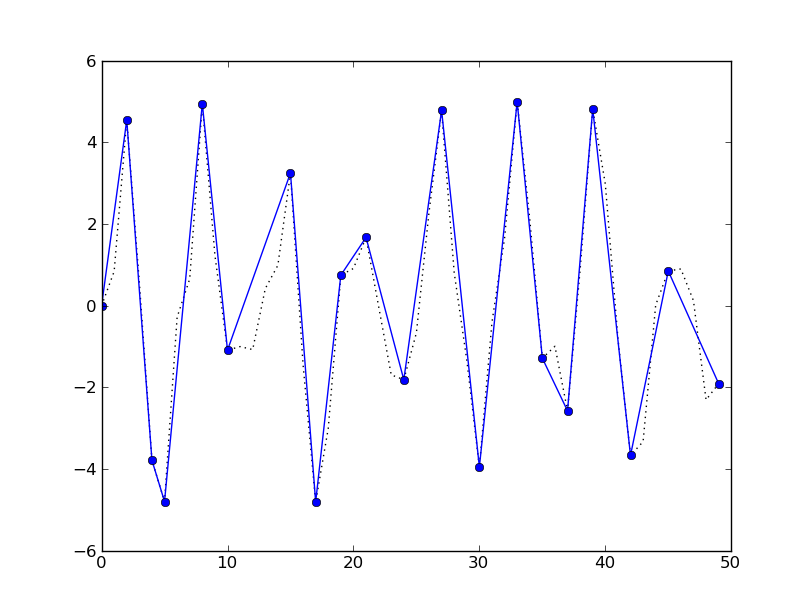
\includegraphics[width=0.4\textwidth]{pip20}}
    \centering
    \caption{Evolução do algoritmo PIP}
    \label{fig:evolucao}
  \end{center}
\end{figure}
\pagebreak

Na figura \ref{fig:evolucao}, conseguimos representar com 20 dos 50 pontos originais (descarte de 60 \% dos dados originais) a série com boa precisão visual, quase se confundindo com a série original para um observador humano. Compressões ainda melhores podem ser alcançadas dependendo da forma geral da série considerada. No apêndice \ref{chap:aproximacao}, pode-se visualizar a representação de uma série original de um mês de dados, com 8582 pontos sendo reduzida para apenas 300 pontos (descarte de aproximadamente 99.97\% dos pontos originais), com uma boa aproximação visual.


\section{Cálculo de distâncias}
Em~\cite{Fu2008} são apresentados testes comparativos com três abordagens diferentes para o cálculo de distâncias entre pontos: distância vertical, distância perpendicular e distância euclidiana. Constatou-se que a distância vertical apresentava os melhores resultados, e portanto, foi a escolhida para este trabalho.

Na figura \ref{fig:vertical-distance} podemos capturar a ideia por trás do cálculo da distância vertical. Os pontos $p1$ e $p2$ representam PIPs previamente escolhidos e o ponto $P3$ um candidato a ser promovido a PIP.
Este método incorpora a intuição de que flutuações verticais são mais importantes para um observador humano.

Em termos práticos, é utilizada a equação \ref{eq:vd} para calcular a distância entre pontos no algoritmo. Podem ser utilizadas técnicas de geometria analítica para se chegar na equação \ref{eq:vd} para o cálculo de distância vertical.

\begin{equation}
\label{eq:vd}
VD(p_{3}, p_{c}) = \mid y_{3} - y_{c} \mid = \mid \Bigg( y_{1} + (y_{2} - y_{1})\bigg(\frac{ x_{3} - x_{1} }{x_{2} - x_{1}}\bigg) \Bigg) - y_{3} \mid
\end{equation}

\begin{figure}[h!]
  \begin{center}
    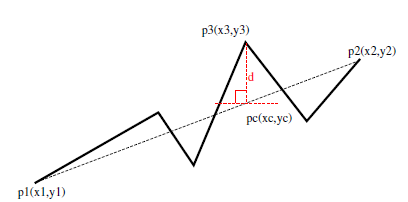
\includegraphics[width=0.6\textwidth]{vertical_distance}
    \centering
    \caption{Distância vertical.}
  \label{fig:vertical-distance}
  \end{center}
\end{figure}

\section{Pseudo-algoritmo}
\label{sec:pseudo-algoritmo}
Pseudo-algoritmos tem seu papel fundamental em estabelecer as macro operações que devem ser realizadas para a resolução de um problema, independente de linguagem de programação, facilitando o entendimento do leitor e o endereçamento de algumas observações sobre o método.

A entrada do algoritmo esperada é uma lista de pontos da série temporal original. Sua saída é um subconjunto desses pontos, que supostamente deveriam ser os mais significativos para um observador humano.

Nas linha 1 e 2 inicializamos a lista de PIPs com o primeiro e último pontos da série. O bloco delimitado pelas linhas 3 a 6 itera sobre os pontos de entrada procurando pelo próximo ponto mais significativo a cada iteração. É importante perceber que a cada iteração são promovidos a PIP apenas um ponto, pois devemos considerar séries temporais por inteiro para não cair em ótimos locais.

\begin{algorithm}[h!]
  \caption{Pseudo-algoritmo Perceptually Important Points}
  \label{alg:PIP1}
  \begin{algorithmic}[1]
  \REQUIRE Lista de pontos da série original $INPUT[1..n]$ ordenada 
  \ENSURE Lista de PIPs $PIP[1..n]$
  \STATE $PIP[1] \Leftarrow INPUT[1]$
  \STATE $PIP[2] \Leftarrow INPUT[n]$
  \REPEAT
    \STATE Selecionar ponto $P-MAX$ de $INPUT$ com maior distância a pontos adjacentes da lista de PIPs. 
    \STATE Inserir $P-MAX$ em $PIP$
  \UNTIL {tenham sido escolhidos n pontos de $INPUT[1..n]$}
  \RETURN $PIP$
  \end{algorithmic}
\end{algorithm}

O pseudo-algoritmo \ref{alg:PIP1} retorna sempre a mesma lista com todos os pontos originais, ainda que a ordem com que sejam escolhidos os pontos revele a importância de cada ponto, a resposta é sempre a mesma, a série original.
Pequenos ajustes podem ser considerados para deixar o algoritmo mais útil em termos práticos. Um deles é definir uma condição de parada para retornar apenas os $k <= n$ pontos mais importantes, exemplificado pelo pseudo-algoritmo \ref{alg:PIP2}.

\begin{algorithm}[h!]
  \caption{Pseudo-algoritmo Perceptually Important Points 2}
  \label{alg:PIP2}
  \begin{algorithmic}[1]
  \REQUIRE Lista de pontos da série original $INPUT[1..n]$ ordenada
  \REQUIRE $k$ pontos a serem escolhidos
  \ENSURE Lista de PIPs $PIP[1..k]$
  \STATE $PIP[1] \Leftarrow INPUT[1]$
  \STATE $PIP[2] \Leftarrow INPUT[n]$
  \REPEAT
    \STATE Selecionar ponto $P-MAX$ de $INPUT$ com maior distância a pontos adjacentes da lista de PIPs. 
    \STATE Inserir $P-MAX$ em $PIP$
  \UNTIL {tenham sido escolhidos $k$ pontos de $INPUT[1..n]$}
  \RETURN $PIP$
  \end{algorithmic}
\end{algorithm}

\subsection{Análise de Complexidade}
Pelo pseudo-algoritmo \ref{alg:PIP1}, podemos observar que as linhas 1, 2 e 7 são executadas em tempo constante. Para fins de análise de complexidade podemos portanto, eliminá-las do cálculo. O bloco delimitado pelas linhas 3 a 6 representam o maior tempo de computação e por isso devemos analisá-lo com mais cuidado.

Na linha 4 são selecionados pontos com maior distância a pontos adjancentes da lista atual de PIPs. Como a cada iteração são promovidos a PIP apenas um ponto e na inicialização já escolhemos dois destes -- primeiro e último da série original -- são selecionados a cada iteração, $(n - 2, n - 3, n - 4, ..., 3, 2, 1)$ pontos para comparação de distâncias. 

Inserir o ponto promovido a PIP na iteração corrente, linha 5, pode ser considerada constante, dependendo da estrutura de dados que se utiliza\footnote{Para a implementação, explicada com mais detalhes no próximo capítulo, as inserções são na verdade $O(log_{32} n)$, pois foi preferida a utilização de \textit{hashsets}, mas que na prática pode ser considerado constante.}.

Sendo assim, a complexidade do algoritmo é dada pelo número de cálculos de distâncias que fazemos no total, e pode ser calculado como:

\[
 \sum_{i=1}^{n - 2} i = \frac{n^2 - 3n + 2}{2}
\]

Deste modo, a complexidade do algoritmo é dada por $O(n^2)$. Já para o pseudo-algoritmo \ref{alg:PIP2}, o mesmo raciocínio pode ser traçado e sua complexidade de tempo é $O(nk)$.

\section{Cálculo de erro}
\label{sec:calculo-erro}
Como destacado na seção \ref{sec:pseudo-algoritmo}, pequenas variantes do pseudo-algoritmo apresentado podem ser implementadas para solucionar algumas dificuldades. Para o pseudo-algoritmo 2 é preciso escolher como entrada o número $k$ de pontos que se deseja resgatar da série original. Normalmente a escolha desse valor não gera bons resultados sem o conhecimento \textit{a priori} da série original.


\begin{figure}[htb!]
  \begin{center}
    \subfloat[Série com 100 pontos, variância muito alta]{\label{fig:alta-variancia}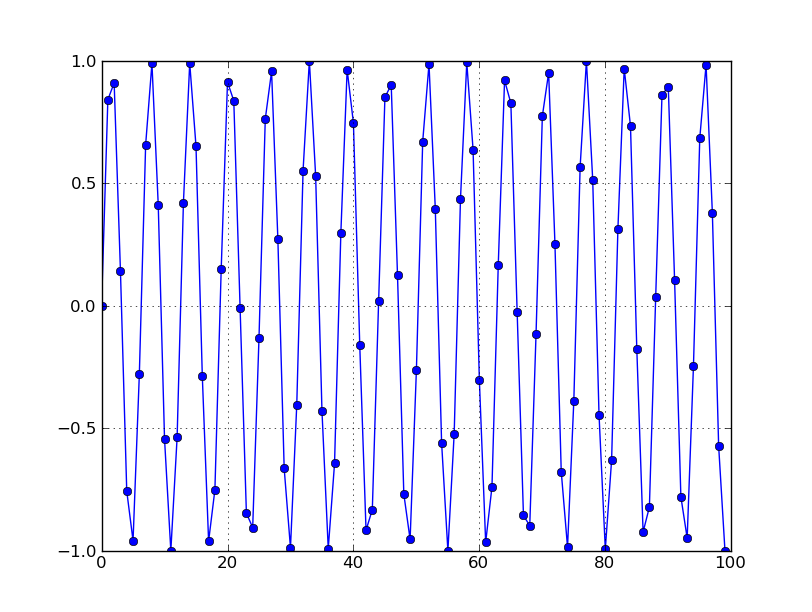
\includegraphics[width=0.4\textwidth]{random-serie}}
    \subfloat[Série com 100 pontos, baixa variância]{\label{fig:baixa-variancia}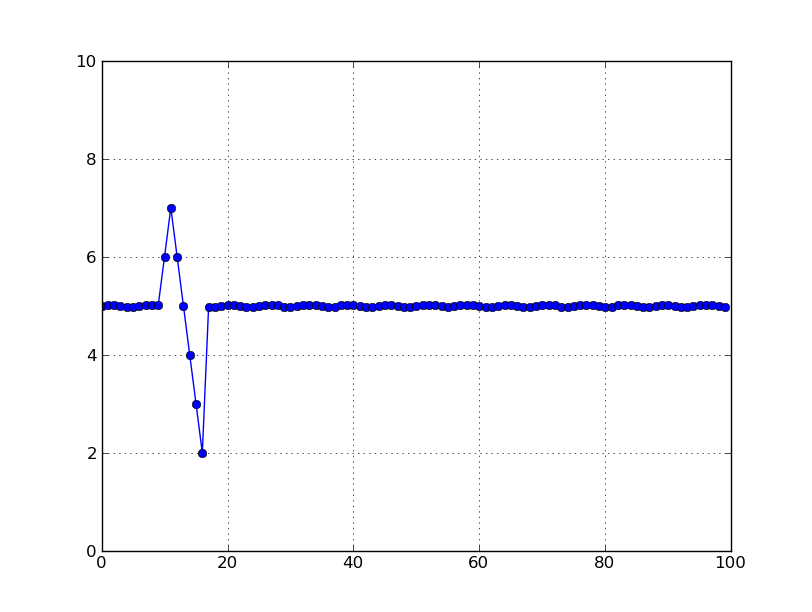
\includegraphics[width=0.4\textwidth]{nice-serie}}
    \centering
    \caption[Variância influencia número de PIPs]{Séries com o mesmo número de pontos podem necessitar de valores bem distintos de PIPs para serem representadas visualmente de modo satisfatório.}
    \label{fig:k-n}
  \end{center}
\end{figure}

Em geral, o valor de $k$ que representa razoavelmente bem\footnote{Como razoavelmente bem, busca-se o conceito subjetivo de similaridade entre duas séries temporais.} a série original não depende do valor de $n$. Para ilustrar tal afirmação, podemos visualizar a figura \ref{fig:k-n}. Na série da figura \ref{fig:alta-variancia}, um número maior de pontos são necessários para representá-la quando comparamos com a figura \ref{fig:baixa-variancia}, uma série mais bem comportada; ainda que as duas possuam a mesma quantidade de pontos no total, no caso 100.

\begin{algorithm}[h!]
  \caption{Pseudo-algoritmo Perceptually Important Points 3}
  \label{alg:PIP3}
  \begin{algorithmic}[1]
  \REQUIRE Lista de pontos da série original $INPUT[1..n]$ ordenada
  \REQUIRE Limite máximo $m$ de pontos a serem escolhidos
  \REQUIRE Erro $\epsilon$ aceitável
  \ENSURE Lista de PIPs $PIP[1..s]$, com $ s <= m$
  \STATE $PIP[1] \Leftarrow INPUT[1]$
  \STATE $PIP[2] \Leftarrow INPUT[n]$
  \REPEAT
    \STATE Selecionar ponto $P-MAX$ de $INPUT$ com maior distância a pontos adjacentes da lista de PIPs. 
    \STATE Inserir $P-MAX$ em $PIP$
  \UNTIL {$m$ pontos de $INPUT[1..n]$ já foram escolhidos ou tenha sido alcançada uma diferença menor que $\epsilon$} 
  \RETURN $PIP$
  \end{algorithmic}
\end{algorithm}

Sendo assim, como não é razoável que a entrada do valor de $k$ seja feita manualmente, é desejável um mecanismo automatizado de inferência sobre o menor valor de $k$ necessário para preservar a forma geral da série original. Para tanto, podem ser utilizadas diferença de mínimos quadrados a cada iteração do algoritmo, dando origem ao pseudo-algoritmo \ref{alg:PIP3}.

\section{Limitações do algoritmo}
\label{sec:limitacoes}
O algoritmo dá mais importância para as grandes flutuações em detrimento de variações mais suaves. O número mínimo de pontos necessários para representar razoavelmente bem uma série está diretamente ligado ao número de picos e vales que a série possui. Para séries com muitos picos e vales com alta amplitude, o algoritmo não consegue uma redução de dimensionalidade significativa.


\chapter{Implementação do algoritmo}
\label{chap:implementacao}
Neste capítulo são apresentadas as ferramentas e técnicas utilizadas para a implementação do algoritmo, testes de performance realizados, dificuldades encontradas e a evolução da implementação durante seu processo de desenvolvimento.

\section{Clojure}
Clojure é uma linguagem de propósitos gerais, dinâmica e funcional, lançada em 2007, por Rich Hickey.
Por se tratar de um dialeto de Lisp\footnote{Lisp (LISt Processing) teve sua primeira especificação em 1958 e foi originalmente pensada como uma notação matemática prática para programas de computador, influenciada pelo Cálculo-$\lambda$ de Alonzo Church. A linguagem ainda é uma das linguagens mais antigas ainda utilizadas largamente no momento da escrita deste texto.}, Clojure foi criada com o intuito de preservar o caráter funcional e poderoso de Lisp para resolver problemas atuais como concorrência e paralelismo numa roupagem mais moderna.

Como se trata de uma implementação do paradigma funcional, a computação dos dados é encarada como avaliações de funções matemáticas, que favorecem o fraco acoplamento entre módulos e incentiva o uso de recursões evitando efeitos colaterais, uma vez que dados são considerados imutáveis nessa linguagem.

Para este trabalho foi utilizada a última implementação estável\footnote{Foi utilizada a versão 1.2, disponível em http://clojure.org/downloads. Último acesso em 20 de novembro de 2010.} da linguagem Clojure no momento da escrita deste texto.


\section{Desenvolvimento}
Preocupações como performance e corretude permearam o processo e técnicas de desenvolvimento ágil como TDD (Test Driven Development)\footnote{Test Driven Development consiste em um processo de desenvolvimento de software em que testes são escritos antes do desenvolvimento do código em si, facilitando o entendimento e condução do processo de raciocínio sobre o problema, além de contribuir como documentação do código.} foram utilizadas durante sua execução.

Todas as funções criadas acompanham testes unitários. Tais testes não garantem totalmente que o código é  correto, mas oferecem um meio de assegurar que alguns casos previamente pensados em que o algoritmo poderia falhar estão cobertos e uma garantia maior pode ser dada para futuros usuários e mantenedores do código.

Nenhuma particularidade do sistema em que foi incorporado este algoritmo -- descrito no capítulo \ref{chap:holmes} -- foi incluída na implementação. Deste modo, o mesmo código pode ser encarado como uma caixa preta e pode ser incorporado em outro sistema com facilidade. Como a linguagem Clojure é compilada para a JVM (Java Virtual Machine), o código também pode ser executado na maioria dos sistemas operacionais existentes atualmente.

\section{Performance}
Apesar do algoritmo apresentado no capítulo \ref{chap:pip} não representar muitas dificuldades de entendimento, implementá-lo de uma forma eficiente requereu pesquisa sobre as estruturas de dados adequadas e detalhes da linguagem para a realização da tarefa.

A implementação do código passou por diversas modificações para atender aos requisitos de performance exigidos pelo projeto. Foram desenvolvidas três versões -- incluídas no Apêndice -- e suas evoluções serão brevemente descritas na próxima seção.

\subsection{Otimizações}
\subsubsection{Versão 1}
A primeira versão do algoritmo -- anexo \ref{chap:versao1} -- foi desenvolvida sem grandes otimizações. Não foi utilizado nenhum mecanismo de cache de resultados intermediários, nem testes muito robustos.

Nesta versão foram definidas as estruturas de dados a serem utilizadas. Para a lista de entrada, se preferiu utilizar \textit{vectors}, que possuem complexidade $O(1)$ para acesso aleatório. Durante o processamento, mantém-se um \textit{vector} que cresce a cada iteração, com os índices na série original para os PIPS escolhidos. Como durante o processamento, são armazenados apenas os índices -- ao invés da combinação $(x, y)$ de cada ponto -- ao se calcular as distâncias são necessários acessos aleatórios a série original para se buscar os pontos. A cada iteração, o \textit{vector} de PIPs é ordenado.

Como os tempos de execução apresentados ficaram bem aquém do desejado, a implantação em um software real -- um dos objetivos pretendidos com esse trabalho, apresentados na seção \ref{sec:objetivos} -- se tornou impeditiva.  Foi necessário, portanto, o desenvolvimento de uma versão de melhor desempenho.


\subsubsection{Versão 2}
Para a segunda versão foram implementadas algumas melhorias. A mais importante de todas se deveu a percepção de que cálculos de distância eram repetidos desnecessariamente. Foi buscada, deste modo, uma solução de cacheamento dos resultados e para tanto, utilizou-se a função \textit{memoize} da linguagem Clojure, que contribuiu para a melhora significativa no tempo de execução.

A cada iteração são armazenados os intervalos entre pips em um \textit{hashset}. A vantagem de se armazenar os intervalos é que os mesmos podem ser avaliados em paralelo -- dependendo de uma sincronização no término para se analisar a melhor distância -- apesar de não ter se utilizado nenhuma espécie de paralelismo nessa versão. Com essa alteração, a necessidade de se ordenar a lista de PIPs a cada iteração passou a inexistir. 

A escolha de um \textit{hashset} se deve a dois motivos. O primeiro deles é que se pode garantir que se a entrada possuir pontos duplicados, estes não aparecerão na saída do algoritmo. O segundo motivo é que como os intervalos são divididos a cada iteração, precisamos redefinir a lista de intervalos, retirando o intervalo anterior, criando dois novos intervalos, no ponto em que o novo PIP foi encontrado. Acessos aleatórios em \textit{hashsets} ocorrem em tempo $O(log_{32}n)$, que na prática pode ser considerado constante.


Como são processadas listas muito extensas e sua avaliação pode ser custosa, optou-se também nesta versão por se utilizar \textit{lazy sequences}\footnote{Para maiores detalhes sobre o conceito de \textit{lazy sequences}, veja~\cite{programmingclojure}}. Como muitos programas escritos em Clojure envolvem computação de listas, a linguagem fornece esse mecanismo para se construir expressões complexas e extensas que só são avaliadas quando realmente são necessárias. Listas infinitas podem ser definidas com esse recurso.

Outra melhoria surgida nessa versão se deu ainda com relação ao cálculo de distâncias. Como são efeituados muitos cálculos de distâncias, foi buscada nessa versão uma implementação mais eficiente. Para isso, substituiu-se o uso da função \textit{abs} do pacote \verb+clojure.contrib.generic.math-functions+ pela versão mais performática da função \textit{abs}, do pacote \verb+clojure.contrib.math+.

Como Clojure é uma linguagem construída por cima da linguagem Java, casting para tipos primitivos para esta linguagem -- discutido em~\cite{practicalclojure}, onde podem ser encontrados outras técnicas para se aumentar o desempenho de programas em Clojure -- também foram adicionados.


\subsubsection{Versão 3}
A versão 3, última desenvolvida, é a que oferece o menor tempo de execução dentre todas as anteriores.
Ao invés de definirmos nossas \textit{lazy sequences}, foi preferida a utilização da função \textit{iterate}, disponível no \textit{core} da linguagem. A função \textit{iterate} recebe como parâmetro uma função e um parâmetro adicional. No momento de sua chamada, a função passada como argumento é executada com o argumento adicional e a sua saída é aplicada a mesma função. O comportamento pode ser continuado indefinidamente. Isso evita muitas trocas de contexto e avaliações de listas muito extensas previamente.

Fez-se uso de mais \textit{lazy sequences} onde necessário e ganhos de performance consideráveis foram conseguidos quando casting para tipos primitivos foram acrescentados no código.

\subsubsection{Testes de performance}
Para comparar a evolução das implementações foram executadas as três versões em ambiente controlado para séries aleatórias e comparados seus tempos de execução.

A máquina utilizada possui as seguintes configurações:
\begin{itemize}
\item Processador: Intel Celeron processor 560, 2.13 GHz, 1 MiB L2 cache
\item Memória Principal: 1 GiB
\item Sistema Operacional: Ubuntu Linux versão 10.04
\end{itemize}

Na tabela \ref{tab:tempos-100} é possível ver um resumo dos tempos de execução para testes realizados com séries aleatórias -- para não privilegiar nenhuma das versões -- de 100 pontos e 1000 pontos. Foram executadas 500 rodadas para cada valor de PIPs e tirada sua média para atender a Lei dos Grandes Números e garantir uma baixa variância nos resultados. Pode-se observar que a Versão 1 destoa bastante das outras duas versões.

\begin{table}[htb!]
  \begin{center}
      \begin{tabular}{ | c | c | c | c | }
      \hline
      \multicolumn{4}{|c|}{Tempos de execução} \\
      \hline
      Número de PIPs & Versão 1 & Versão 2 & Versão 3 \\ \hline
      4 & 7.49943    & 1.8605996 & 0.6156479 \\ \hline
      10 & 26.238653 & 2.321418  & 1.0887681 \\ \hline
      20 & 54.226994 & 4.5783596 & 1.3933954 \\ \hline
      30 & 84.99333  & 5.6005797 & 2.06694   \\ \hline
      40 & 115.92436 & 7.35721   & 3.0876982 \\ \hline
      50 & 145.32526 & 9.438611  & 3.6283286 \\ \hline
      60 & 156.99683 & 12.641098 & 4.9837728 \\ \hline
      70 & 171.61131 & 14.659222 & 5.6078625 \\ \hline
      80 & 174.81184 & 15.915979 & 7.315132  \\ \hline
      90 & 189.28699 & 18.447191 & 8.141004  \\
      \hline
      \end{tabular}
  \end{center}
  \caption[Tempos de execução]{Tempos de execução para as três versões implementadas do algoritmo PIP para séries com 100 pontos. Os tempos estão em milissegundos.}
  \label{tab:tempos-100}
\end{table}


\begin{table}[htb!]
  \begin{center}
      \begin{tabular}{ | c | c | c | c | }
      \hline
      \multicolumn{3}{|c|}{Tempos de execução} \\
      \hline
      Número de PIPs & Versão 2 & Versão 3 \\ \hline
      100 & 239.5926  & 101.20084 \\ \hline
      200 & 342.2604  & 184.52263 \\ \hline
      300 & 396.32697 & 163.0423  \\ \hline
      400 & 538.5814  & 217.53302 \\ \hline
      500 & 706.6794  & 328.58374 \\ \hline
      600 & 952.6192  & 394.18314 \\ \hline
      700 & 1071.5186 & 481.18253 \\ \hline
      800 & 1279.3595 & 561.9523  \\ \hline
      900 & 1397.1849 & 708.9733  \\
      \hline
     \end{tabular}
  \end{center}
  \caption[Tempos de execução para as duas melhores versões]{Tempos de execução para as duas melhores versões implementadas do algoritmo PIP para séries com 1000 pontos. Os tempos estão em milissegundos.}
  \label{tab:tempos-1000}
\end{table}

É possível observar também que a Versão 3 é duas vezes mais rápida que a Versão 2 analisando os valores da tabela \ref{tab:tempos-1000}. Um ganho considerável de performance quando séries com alta dimensionalidade  devem ser processadas. Nas figuras \ref{fig:comp-3-versions} e \ref{fig:comp-2-versions}, podem ser vistos os mesmos dados de forma gráfica.

\begin{figure}[htb!]
  \begin{center}
    \subfloat[Comparação entre os tempos de execução das três versões implementadas. Série original possuía 100 pontos.]{\label{fig:comp-3-versions}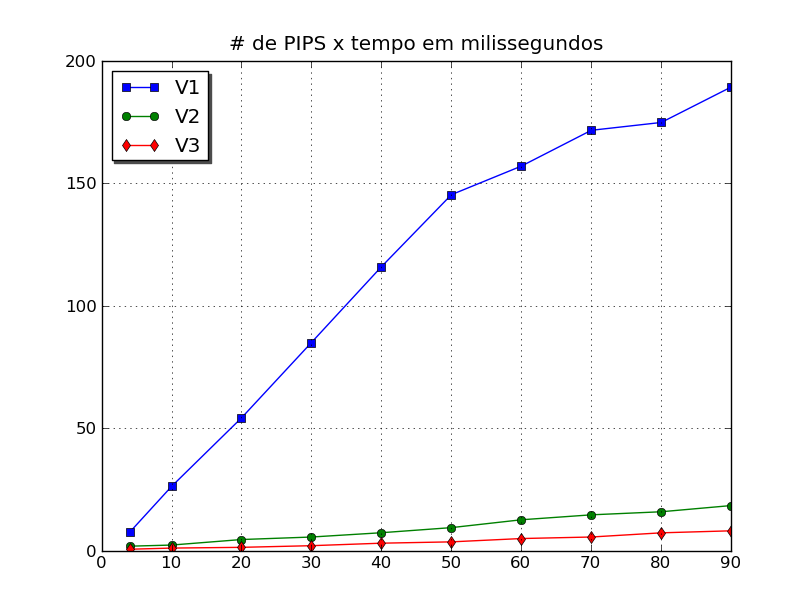
\includegraphics[width=0.5\textwidth]{execution-time-3-versions-100-points}}
    \\
    \subfloat[Comparação entre os tempos de execução das duas melhores versões implementadas. Série original possuía 1000 pontos.]{\label{fig:comp-2-versions}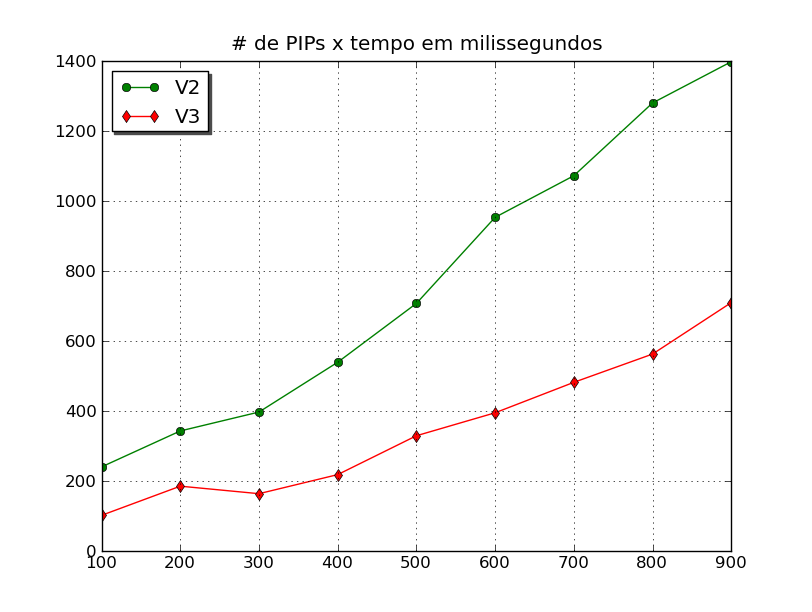
\includegraphics[width=0.5\textwidth]{execution-time-2-versions-1000-points}}
    \centering
    \caption[Comparativo entre as 3 versões implementadas]{Tempos de execução para as implementações do algoritmo PIP}
    \label{fig:comparativo}
  \end{center}
\end{figure}

\chapter{Aplicação em um sistema real}
\label{chap:holmes}

O objetivo da implementação do algoritmo apresentado no capítulo \ref{chap:implementacao} foi permitir sua implantação no sistema de monitoração de datacenters HOLMES, brevemente descrito neste capítulo. 

A integração com o algoritmo PIP e a arquitetura do software envolvida também são discutidas. Ademais, o resultado final é apresentado e em seguida um caso de uso de sucesso é apresentado.

\section{HOLMES}

O dia a dia da equipe de operação de um datacenter envolve entre outras atividades, o acompanhamento em tempo real de informações provenientes de diferentes máquinas e dispositivos. Centenas de métricas precisam ser monitoradas para garantir que o sistema não apresente quedas de serviço ou \textit{downtime}, o que na maioria dos casos pode provocar perdas significativas de faturamento para o mantenedor do datacenter e seu negócio.

O software HOLMES foi criado com o propósito de fornecer aos operadores de datacenters ferramentas para análise e monitoramento de informações em tempo real, favorecendo o aumento de sua consciência situacional, fator crítico em um ambiente em que muitos equipamentos precisam ser monitorados e a correlação entre eventos para a resolução de um dado problema pode ser difícil, mesmo para operadores experientes.

\section{Integração HOLMES e PIP}
Dentre outras funcionalidades, o software possui uma interface de visualização de gráficos. Nessa interface é possível inspecionar gráficos de métricas coletadas ao longo do tempo provenientes dos itens de configuração cadastrados pelos usuários do sistema.

O termo item de configuração é originário da terminologia ITIL\footnote{ITIL, Information Technology Infrastructure Library.} e pode representar um dispositivo físico como roteador, disco rígido, unidade de processamento, ou qualquer outra métrica lógica como protocolo TCP/IP, HTTP, etc.

Itens de configuração são, em geral, cadastrados no sistema pela equipe de operadores do datacenter. Uma vez cadastrados e configurados, os itens de configuração passam a emitir eventos para um barramento central, de onde são coletados e armazenados. Com base nesses eventos, podemos construir suas séries temporais em sua forma mais bruta. 

Devido a propriedade de alta dimensionalidade, essas séries requerem um processamento adicional antes de serem entregues efetivamente para o usuário final, na interface de visualização. É nesta fase que o algoritmo PIP é empregado, com o papel de reduzir a dimensionalidade dos dados originais e oferecer uma visualização que preserva o comportamento e a forma do gráfico da série original.


\subsection{Arquitetura}
O software de monitoração HOLMES possui um barramento central -- módulo Message broker na figura \ref{fig:overview-architecture} -- destino dos eventos provenientes de diversos equipamentos. Esses dados são coletados e enviados para um módulo de armazenamento denominado \textit{storage}, ilustrado na figura \ref{fig:overview-architecture}.

Na figura \ref{fig:overview-architecture} é demonstrada a arquitetura geral do sistema HOLMES, com destaque para os módulos envolvidos na integração.


\begin{figure}[h!]
  \begin{center}
    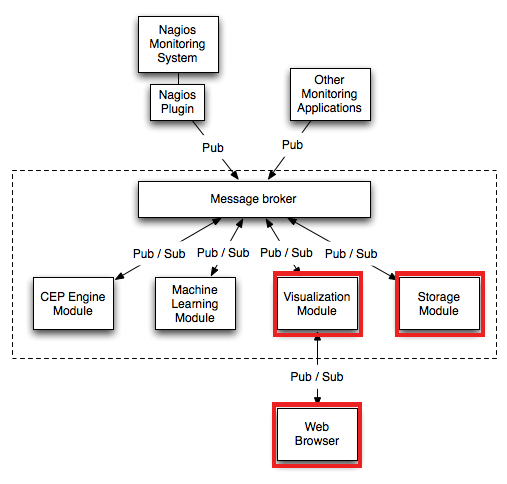
\includegraphics[width=0.6\textwidth]{overview_architecture}
    \centering
    \caption[Arquitetura do sistema HOLMES]{Arquitetura do sistema HOLMES e módulos participantes da integração com o algoritmo PIP}
  \label{fig:overview-architecture}
  \end{center}
\end{figure}

Quando um usuário final requisita uma série temporal através da interface web do sistema HOLMES, o módulo storage é ativado. Os dados originais são coletados e entregues para processamento pelo algoritmo PIP,  devolvidos em seu término\footnote{Os dados são devolvidos em formato JSON (JavaScript Object Notation),  formato de serialização de dados largamente utilizado na Internet.} para o web browser do cliente.

A partir dos pontos perceptivelmente mais importantes no web browser do cliente, seus pontos são entregues finalmente a uma biblioteca Javascript para a plotagem final. Essa estratégia evita que pela rede sejam trafegados todos os pontos originais das séries temporais requisitadas. 

Além disso, ainda que não existissem problemas de banda no tráfego de todos os pontos, outra dificuldade surgiria na etapa de plotagem dos gráficos, no que diz respeito a densidade de pontos. O algoritmo PIP resolve de forma satisfatória essas duas dificuldades.

\subsection{Visualização}
\label{sub:visualizacao}
Para ilustrar o resultado final do que foi exposto até aqui, alguns screenshots foram tirados do sistema HOLMES, que é apenas um codinome para o sistema real: Intelie Event Manager.

As séries temporais que são exibidas para o usuário final estão organizadas na área Histórico do sistema. Na figura \ref{fig:graf-mini}, é possível observar alguns gráficos utilizando o algoritmo PIP. Como o sistema é comercial, alguns nomes foram borrados para manter privacidade de seus clientes. Repare que segundo descrito na seção \ref{sec:limitacoes}, o algoritmo PIP não se comporta muito bem com muitos picos e vales, mas ainda assim apresenta resultados satisfatórios quando o número de PIPs é suficiente, como pode ser observado na figura \ref{fig:tcp-mini}.

\begin{figure}[htb!]
  \begin{center}
    \subfloat[Load mínimo nos últimos 15 minutos]{\label{fig:load-mini}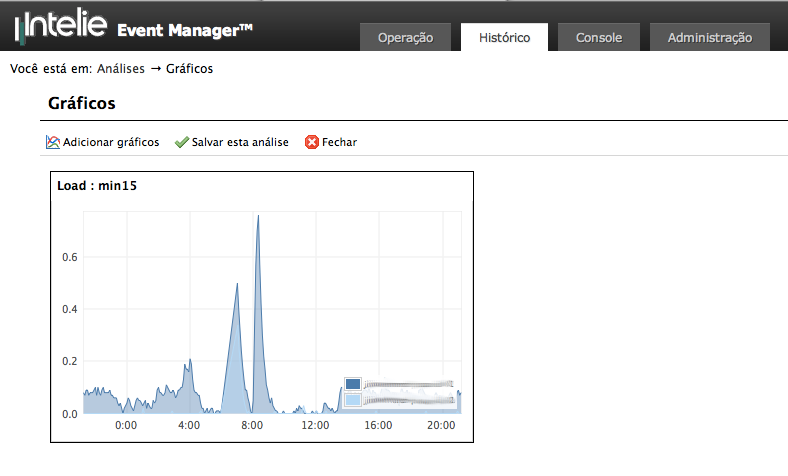
\includegraphics[width=1\textwidth]{load_mini}} \\
    \subfloat[Tempo de resposta do protocolo TCP]{\label{fig:tcp-mini}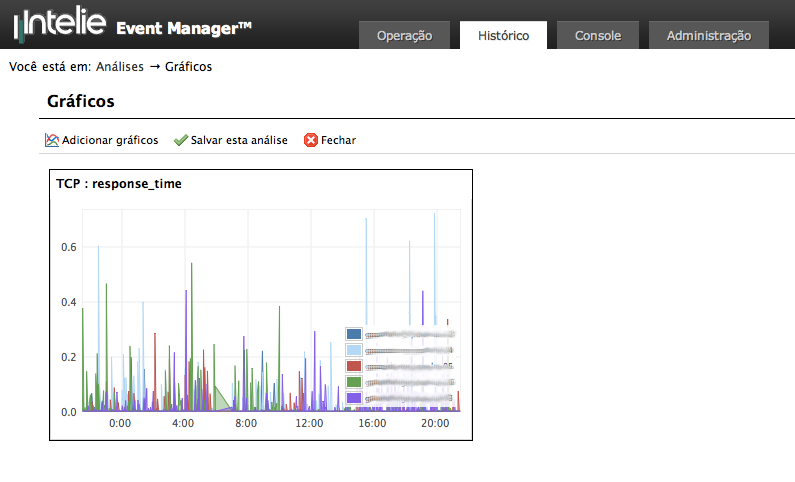
\includegraphics[width=1\textwidth]{tcp_mini}}
    \centering
    \caption{Gráficos gerados a partir do algoritmo PIP no sistema HOLMES}
    \label{fig:graf-mini}
  \end{center}
\end{figure}

\begin{figure}[htb!]
  \begin{center}
    \subfloat[Load mínimo nos últimos 15 minutos]{\label{fig:load-big}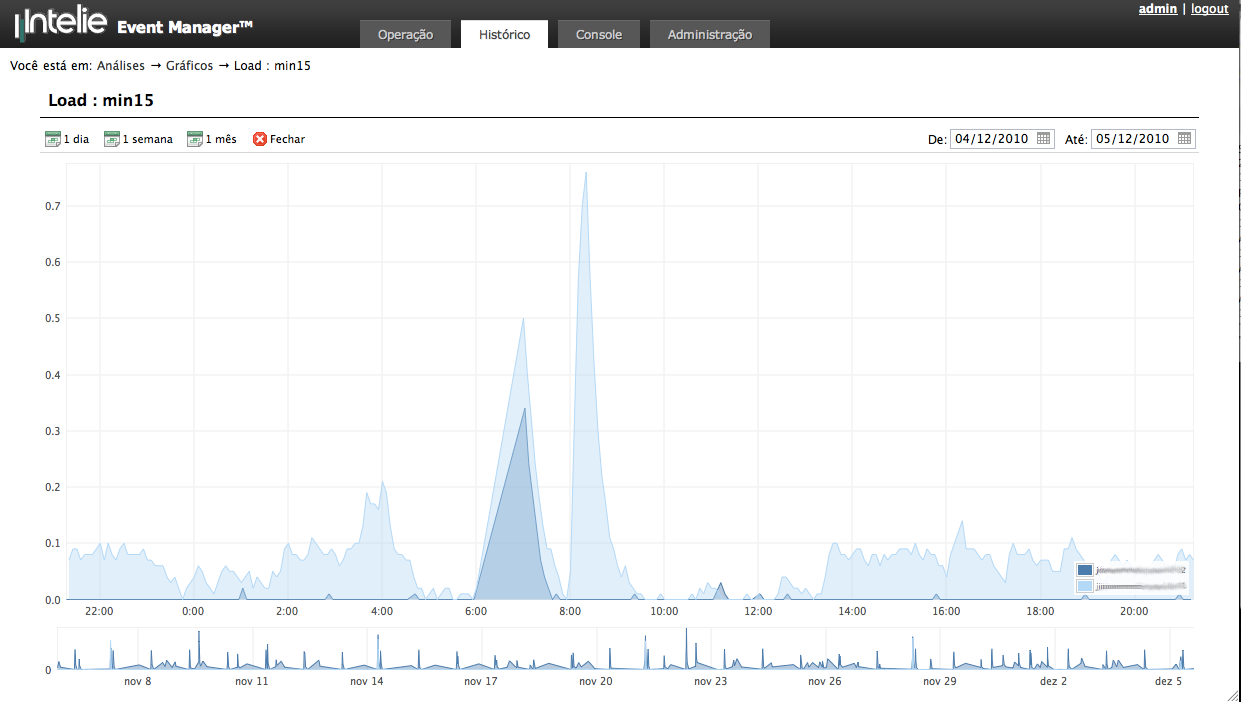
\includegraphics[width=1\textwidth]{load_big}} \\
    \subfloat[Tempo de resposta do protocolo TCP]{\label{fig:tcp-big}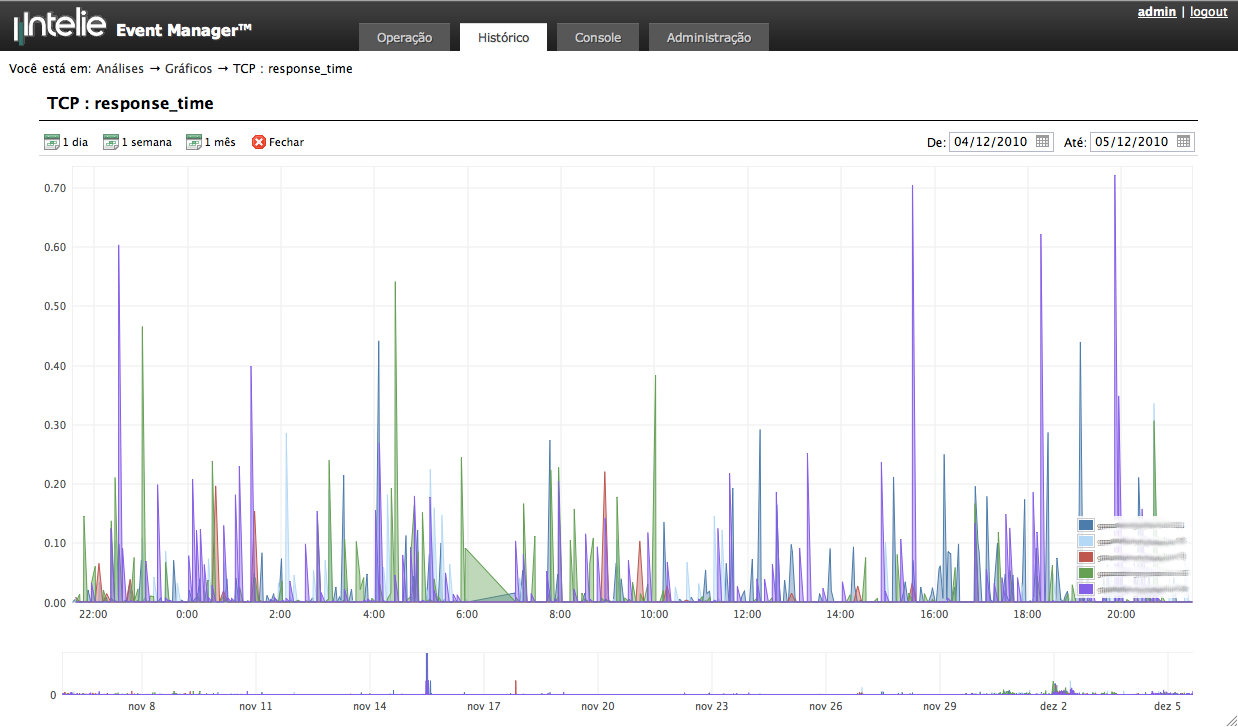
\includegraphics[width=1\textwidth]{tcp_big}}
    \centering
    \caption{Gráficos gerados a partir do algoritmo PIP no sistema HOLMES}
    \label{fig:graf-big}
  \end{center}
\end{figure}

\section{Caso de Uso}
O sistema HOLMES está em uso atualmente em dois grandes datacenters do Brasil: Globo.com e iG.

Versões anteriores do sistema HOLMES contavam com técnicas de média sobre média, brevemente discutidas na seção \ref{sec:time-series-datacenter}, que desfiguravam a forma geral do gráfico, confundindo usuários finais em sua interpretação dos dados.

Operadores destes datacenters manifestaram diminuição no tempo de detecção de falhas de problemas em equipamentos de seus servidores após a implementação da interface de visualização utilizando o algoritmo PIP.

\chapter{Conclusão}
\label{chap:conclusao}
Com o aumento da capacidade de processamento e armazenamento das máquinas seguindo a Lei de Moore, a possibilidade de se lidar com séries temporais cada vez maiores vem crescendo ao longo dos anos. A literatura existente sobre o assunto é extremamente vasta e rica, com aplicações nos mais variados campos do conhecimento humano.

O algoritmo escolhido para esse trabalho tem sido usado em séries temporais do mercado financeiro e aplicações no domínio de datacenters é nova até onde foi possível se investigar.

A relevância deste trabalho se manifesta a partir da aprovação por parte dos usuários do sistema HOLMES, com relatos confirmando a diminuição no tempo de identificação e solução de problemas em ambientes de operação de datacenters.

Apesar dos objetivos definidos para este trabalho -- expostos na seção \ref{sec:objetivos} -- terem sido alcançados com êxito, muitas melhorias no software ainda se fazem necessárias; como um mecanismo para o cálculo de erro e escolha automatizada do número mínimo de pontos -- descritos na seção \ref{sec:calculo-erro} -- para representar a série temporal original, não incluída na versão final da implementação devido o fator tempo. 

Por fim, pode-se endereçar a trabalhos futuros, a integração com outros algoritmos de representação e redução de dimensionalidade na tentativa de se reduzir as limitações do algoritmo \textit{Perceptually Important Points}, além de testes comparativos mais extensos no domínio de datacenters.

\appendix
\lstset{ %
language=[Auto]Lisp,
basicstyle=\footnotesize,
frame=single,
numbers=left,
breaklines=true,
framerule=0.4mm,
showstringspaces=false}

\begin{appendices}
  \chapter{Primeira Versão}
  \label{chap:versao1}
  \lstinputlisting{/home/kaiser/Dropbox/monografia/code/versao1_monograph.clj}

  \chapter{Segunda Versão}
  \label{chap:versao2}
  \lstinputlisting{/home/kaiser/Dropbox/monografia/code/versao2_monograph.clj}

  \chapter{Terceira Versão}
  \label{chap:versao3}
  \lstinputlisting{/home/kaiser/Dropbox/monografia/code/versao3_monograph.clj}

  \chapter{Aproximações}
  \label{chap:aproximacao}
%  \begin{landscape}
  \begin{figure}[htb!]
    \begin{center}
      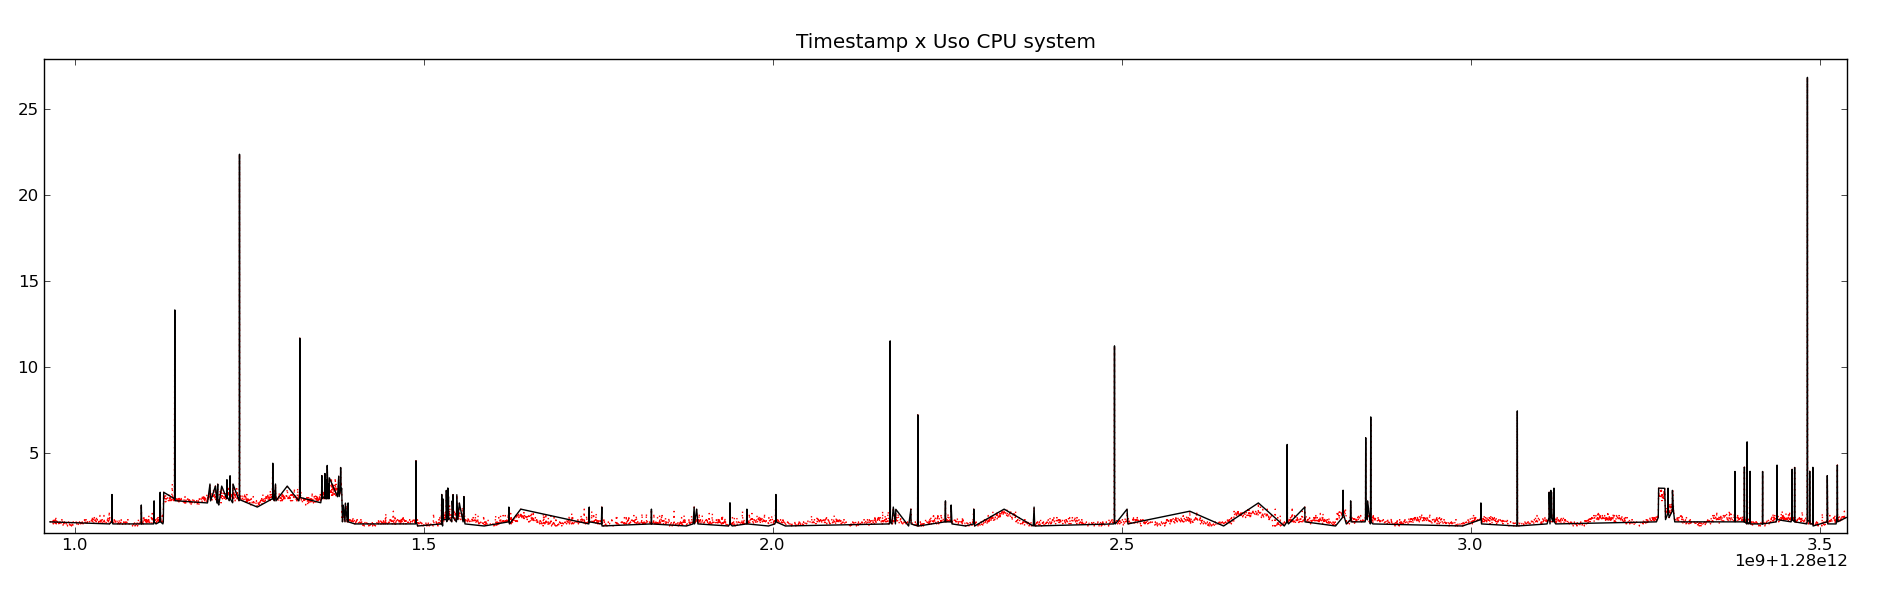
\includegraphics[width=1\textwidth]{timestampxcpu_system_8582_300_hpg-spo-squid-01}
      \centering
      \caption[Série original com 8582 pontos reduzida com PIP para 300 pontos]{Série original -- linha pontilhada em vermelho -- com 8582 pontos representando 1 mês de observações, reduzida com PIP para 300 pontos. Descarte de 99.976\% dos pontos originais.}
    \label{fig:approx1}
    \end{center}
  \end{figure}
%  \end{landscape}

\end{appendices}


\bibliographystyle{unsrt}
\bibliography{references}

\end{document}
